Dal punto di vista organizzativo del progetto \emph{GoBus}, si \`{e} deciso grazie alle esperienze acquisite dal team, di trovare un giusto equilibrio tra il ciclo di vita di un progetto, costituito dalle fasi di ingegnerizzazione e produzione, e il ciclo gestionale costituito invece dalle attivit\`{a} e processi svolti dal team per governare il progetto. Quindi questa fusione di conoscenze ci ha permesso di gestire al meglio il ciclo di vita del progetto. Si \`{e} deciso di seguire le linee guida dettate dal \emph{Project Management Body of Knowledge} che descrive l\rq insieme delle prassi standard per la gestione di progetti cos\`{i} come definite dal “Project Management Institute”. I processi del Project Management descritti nel \emph{PMBOK®} \cite{PMBOK} sono 47 distribuiti in 5 gruppi, in particolare nell’ambito di GoBus sono stati utilizzati per:

\begin{itemize}
	\item {\bf{Inizializzazione}}: Raggruppa i processi necessari a selezionare un progetto in relazione a specifici obiettivi di business e definendo obiettivi e modalit\`{a} di gestione del progetto.
	\item {\bf{Pianificazione}}: Finalizzata a circoscrivere l\rq ambito ed i deliverables del progetto, a definire requisiti di ciascun deliverable e a definire un piano di Project Management contenente tutti i vari piani in dettaglio per la gestione di: tempi, risorse, costi, qualit\`{a}, rischi, comunicazione.
	\item {\bf{Esecuzione}}: Finalizzata a gestire e sviluppare il progetto, produrre i deliverables concordati.
	\item  {\bf{Monitoraggio e Controllo}}: Servono a valutare l\rq avanzamento dei lavori, a gestire eventuali modifiche e a verificare la qualit\`{a} di quanto realizzato.
	\item {\bf{Chiusura}}: Finalizzata a gestire la chiusura del progetto.
\end{itemize}

\subsection{Inizializzazione}
In questa fase \`{e} stato inizializzato il progetto puntando prima a definire il team e identificare gli stakeholder di progetto e successivamente a definire Business need e strategie da attuare. Per quanto riguarda il team \`{e} stato creato come deliverable il team contract dove sono state definite alcune regole che riguardano comunication e people management, mentre per gli stakeholder \`{e} stato creato un registro dove memorizzare i vari stakeholder del progetto nel tempo e i loro contatti. Dopo aver creato le basi del team di progetto si \`{e} definito come lo Statement of work che racchiude in se le caratteristiche che dovr\`{a} avere il progetto, ovvero le Business needs, le funzionalit\`{a} chiave e il piano strategico che si punta ad ottenere con GoBus. Per quanto riguarda i Bussiness needs come definito anche da ITIL® \cite{ITIL}, \emph{``ogni servizio deve avere una giustificazione''} per questo motivo all’interno di un progetto \`{e} fondamentale identificarli e renderli protagonisti della strategia di sviluppo del progetto. Tra i Business needs citati nello Statement of work abbiamo ad esempio la fruibilit\`{a} dell\rq informazione, vitale \`{e} la knowledge sharing, ovvero la diffusione della conoscenza e informazione tramite il servizio offerto. Dallo Statement of work \`{e} gi\`{a} possibile iniziare a tirar fuori i requisiti funzionali che saranno successivamente identificati meglio all\rq interno del Requirements Analysis Document.

\subsection{Pianficazione}
Nella fase di Planning si \`{e} racchiuso tutto il lavoro di pianificazione per quanto riguarda le attivit\`{a} di progetto da svolgere. Passo fondamentale \`{e} stato la realizzazione del Software Project Management Plan (SPMP). Per la realizzazione di quest\rq ultimo si \`{e} seguito quello che \`{e} lo standard ISO-IEC-IEEE 16326-2009 cercando di rispettare le voci specificate dallo standard.
Il Software Project Management Plan (SPMP) \`{e} stato realizzato attraverso la collaborazione tra i quattro componenti del team, sulla base delle esperienze maturate dai singoli e da tecniche facilitative quali brainstorming.
In particolare ci si \`{e} basati sul documento di Statement of Work dal quale \`{e} stato possibile comprendere le deliverables del progetto da realizzare incluse nell\rq apposita sezione dell\rq SPMP.
Ovviamente il documento \`{e} stato aggiornato pi\`{u} volte con l\rq avanzare del progetto. In questo senso, lo scope del progetto \`{e} stato ricavato a partire proprio dalle business needs elaborate e descritte nel documento.
A partire da queste si \`{e} quindi potuto elaborare una descrizione dello scope che \`{e} stata inclusa nell\rq SPMP ed in documenti quali il RAD.
Nella sezione Project Context dell\rq SPMP si \`{e} proceduto alla descrizione del modello di processo adottata nell\rq ambito del progetto e alle modalit\`{a} di miglioramento del processo.
Importante \`{e} stata la definizione degli strumenti e delle infrastrutture necessarie al progetto. Tra questi rientrano appunto dei tool collaborativi quali Google Drive, per la comunicazione quali Google Groups, Skype oltre che vari tools di sviluppo software.
Viene inoltre definito il ruolo del Project Manager nell\rq ambito del progetto. Tale ruole viene ricoperto a turno dai diversi membri del team.
In contemporanea, per consentire un adeguato Management dello Scope di progetto, si \`{e} realizzato un Requirements Management Plan (RMP), sottoinsieme dell\rq SPMP. Lo scopo di tale documento \`{e} specificare le modalit\`{a} di raccolta requisiti ed analisi. 
Nel dettaglio, si sono specificati quelli che sono gli strumenti per la specifica dei requisiti, quali ad esempio Word ed Excel, tecniche di Elicitation quale la preparazione di interviste e tecniche di Analisi dei requisiti quali brainstorming, prototipazione, prioritizzazione etc.
Nel nostro caso per la raccolta dei requisiti si \`{e} scelto di effettuare delle interviste piuttosto che utilizzare una tecnica etnografica che avrebbe portato via tempo e non avrebbe condotto a risultati immediati, soprattutto in vista del fatto che l\rq app finale \`{e} orientata ad una vasta gamma di utenti. Non \`{e} stato possibile effettuare nemmeno alcun benchmarking rispetto ad altri progetti simili, per via delle nostre esigue esperienze.
Per la prioritizzazione dei requisiti si \`{e} deciso di utilizzare tre categorie di valutazione qualitative: alto, medio, basso. In modo da individuare immediatamente su quali requisiti e funzionalit\`{a} concentrare gli sforzi. 
Se pur lo scope di progetto \`{e} risultato chiaro sin dalle primissime fasi, fondamentale \`{e} stata la definizione di un Change Management per quanto concerne i requisiti. In particolare nella definizione delle figure preposte all\rq accettazione dei cambiamenti e alla valutazione dell\rq impatto che tali cambiamenti hanno sul sistema.
In ultimo si \`{e} definita e specificata una Requirements Traceability Matrix (RTM) che ci consente di tener traccia dei requisiti per tutta la durata del progetto e quindi poter verificare l\rq impatto di un cambiamento sul sistema. 
All\rq interno della stessa si va a definire il codice del requisito, un rationale che motiva il requisito, la fonte, l\rq autore, la data di raccolta, una priorit\`{a} ed uno status, oltre a vari riferimenti del requisito all\rq interno dei diversi documenti e del codice sorgente.
Il seguente \`{e} un esempio di macro requisito specificato nell’RTM:
\\
\begin{figure}[h]
\centering
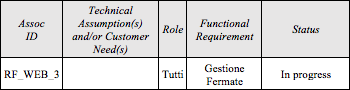
\includegraphics[scale=.7]{img/1.png}
\label{fig:cd}
\end{figure}
\\
\begin{figure}[h]
\centering
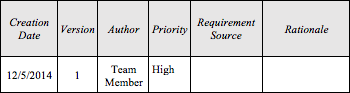
\includegraphics[scale=.7]{img/2.png}
\label{fig:cd}
\end{figure}
\\
\begin{figure}[h]
\centering
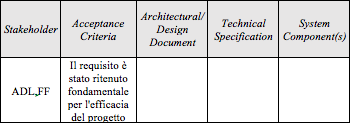
\includegraphics[scale=.7]{img/3.png}

\label{fig:cd}
\end{figure}
\\
\begin{figure}[h]
\centering
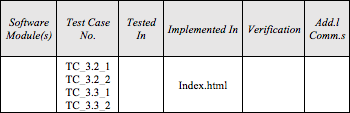
\includegraphics[scale=.7]{img/4.png}
\caption{Esempio di RTM}
\label{fig:cd}
\end{figure}
\\
Nella tabella ADL e FF rappresentano rispettivamente il prof. Andrea De Lucia e la proff.ssa Filomena Ferrucci ritenuti nell\rq ambito del progetto stakeholder e top management.
Il Requirements Management Plan \`{e} risultato quindi fondamentale per la definizione del RAD, descritto nella sezione Software, in cui vengono appunto specificati tutti i requisiti.
Con la realizzazione dell\rq RMP e parallelamente all’attivit\`{a} di raccolta requisiti si \`{e} proceduto alla redazione del Software Configuration Management Plan (SCMP). Questa scelta risiede nel fatto che il RAD risulta essere il documento fondante del progetto e che appunto forma la base da cui partire. Modifiche a requisiti dovrebbero essere approvati mediante accettazione formale, soprattutto se queste possono impattare gravemente sul sistema.
Per cui prima di procedere alla realizzazione del RAD \`{e} buona norma predisporre un SCMP. 
Viste le ridotte dimensioni del team lo stesso \`{e} incaricato di valutare i cambiamenti da apportare a Configuration Items baselined.
Nello specifico, il Project Manager di turno \`{e} il Configuration Manager designato. Il ruolo di sviluppatore e auditor \`{e} di volta in volta assegnato a membri del team diversi.
Change Control Board \`{e} l\rq intero team che \`{e} incaricato di valutare l\rq impatto e schedulare le modifiche da apportare.
I Configuration Items (CI) vengono quindi decisi nelle primissime fasi del progetto. Tra questi \`{e} risultato necessario includere: 
\begin{figure}[h]
\centering
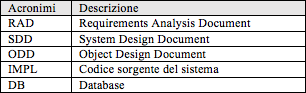
\includegraphics[scale=.7]{img/5.png}
\caption{Configuration Item}
\label{fig:cd}
\end{figure}
Ovviamente altri CI possono essere inclusi in ogni momento se ritenuto necessario.
Le richieste formali di cambiamento non sono schedulate, e possono quindi essere fatte in qualsiasi momento. Questa scelta \`{e} motivata dal fatto che lo scope del progetto \`{e} ben chiaro cos\`{i} come i requisiti iniziali, per cui modifiche in corso d\rq opera non vanno a stravolgere il sistema progettato.
Fondamentale \`{e} risultata anche la scelta di un repository software sul quale \`{e} possibile tener traccia delle diverse versioni del software, tra cui appunto le versioni baselined. Lo stesso DB verr\`{a} caricato su repository insieme al codice sorgente e le versioni baselined verranno specificate in appositi documenti, cos\`{i} come le richieste formali di cambiamento e delle modifiche apportate alle baseline.
Ovviamente per modifiche ai requisiti si pu\`{o} far riferimento alla sezione di Change Management specificata nell\rq RMP.
Per la redazione del documento si \`{e} fatto riferimento allo Std. 828-1990 in versione down-tailored viste le dimensioni del progetto.
Il Configuration Management Plan consente quindi di mantenere il progetto all\rq interno dello scope e questo \`{e} il motivo per il quale si \`{e} deciso di svilupparlo in contemporanea con la fase di raccolta requisiti consentendo l\rq implementazione del Configuration Management come funzione di progetto.
Con la raccolta requisiti e l\rq analisi di quest\rq ultimi si \`{e} quindi definito la versione relativa del RAD come baselined.
A partire da questa, insieme con lo scope definito in precedenza, si \`{e} proceduto alla realizzazione di una baseline dello scope di progetto in base al quale valutare gli avanzamenti, dapprima con la realizzazione di una Work Breakdown Structure (WBS) ed in seguito con la realizzazione di uno scheduling delle attivit\`{a}.
Per quanto riguarda la WBS, essa \`{e} stata realizzata mediante brainstorming da parte del team prendendo in considerazione lo scope, i requisiti, le conoscenze del team e procedendo per analogia rispetto ad altre WBS costruite in precedenza.
In particolare \`{e} stato utile un misto di approcci di visualizzazione tra funzionale e per componenti di progetto. Nel primo caso ci si \`{e} serviti dei 5 process groups definiti dal PMI nel PMBOK 5, nel secondo caso ci si \`{e} basati sia su documenti di Management che tipici dell\rq Ingegneria del Software.
Questo approccio ci ha consentito di rilevare alcuni dettagli non rilevati in prima battuta. 
Il formato finale della WBS \`{e} di tipo gerarchico. Ovviamente si tratta di una WBS grossolana che verr\`{a} raffinata con l’avanzare del progetto. Non risulta infatti critica la definizione con largo anticipo dei task e delle responsabilit\`{a} sui singoli task se non per stima dei tempi di progetto.
La \emph{figura 3} mostra la WBS elaborata.

\begin{figure*}[tp]
\centering
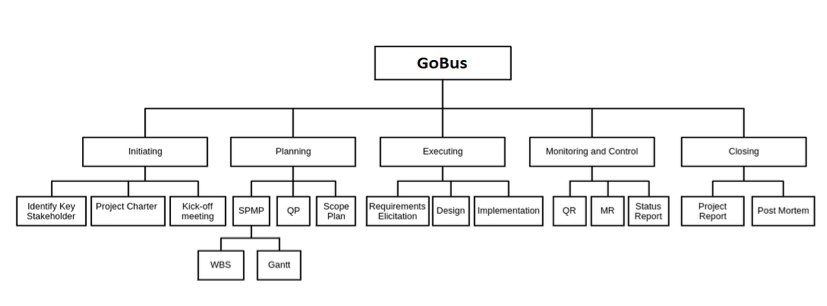
\includegraphics[scale=.6]{img/6.png}
\caption{WBS}
\label{fig:cd}
\end{figure*}

Sulla base di quest\rq ultima si \`{e} poi passato alla realizzazione dello scheduling delle attivit\`{a}.
Come gi\`{a} accennato in precedenza alcune attivit\`{a} sono state effettuate in contemporanea con altre. Dall\rq esperienza maturata su progetti precedenti si \`{e} riuscito stabilire una durata approssimativa delle diverse attivit\`{a}, soprattutto relative alla fase di initiating e planning.
Inoltre \`{e} stato considerato uno slack time aggiuntivo per le diverse attivit\`{a}.
Per la schedulazione (presente nell\rq SPMP in allegato) si \`{e} tenuto principalmente conto delle deadlines imposte da Score-IT e dagli impegni relativi allo studio di ogni componente del team.
Si \`{e} inoltre tenuto conto anche della presenza, fondamentale, di un corso di sviluppo applicazioni mobili al secondo semestre, per cui la fine del progetto \`{e} stata prevista per il 30/06/2015.
Sia la WBS che lo scheduling vengono specificate nella sezione Project Planning dell’SPMP. In questa sezione viene inoltre specificato, tra i vari aspetti, quello legato al training.
Infatti la realizzazione di un\rq App per Windows Phone comporta l\rq apprendimento da parte dei membri del team di tecnologie non conosciute al momento, tra cui C\# e la conoscenza dell\rq ambiente di sviluppo .NET. In contemporanea con la realizzazione della WBS si \`{e} proceduto con la realizzazione del Quality Plan (QP). Il Quality Plan (QP) \`{e} stato redatto in questa fase del progetto in quanto \`{e} importante avere uno scope chiaro e dei requisiti funzionali e non funzionali chiari in modo da rispettare degli obiettivi di qualit\`{A} che si relazionino ai requisiti. Per cui la base di tale QP \`{e} stato il RAD, l’SPMP e lo SoW.
Lo standard di riferimento \`{e} stato l’ISO/IEC 9126 che definisce un modello di qualit\`{A} del software. In particolare, tale standard definisce sei categorie di qualit\`{a}, ulteriormente suddivise in sotto categorie secondo una struttura gerarchica. Si \`{e} deciso di dare una forte rilevanza all\rq aspetto della funzionalit\`{a} soprattutto per quanto riguarda l\rq accuratezza.
Questo consentir\`{a} agli utenti finali di poter ottenere le informazioni nel modo pi\`{u} dettagliato e preciso possibile, tenendo ovviamente conto di aspetti collegati alla sicurezza delle informazioni sensibili dell\rq utente ed una adeguatezza delle funzionalit\`{a} a quello che \`{e} lo scopo del sistema.
Si \`{e} deciso inoltre di garantire un alta operabilit\`{a} garantendo all\rq utente un alto controllo delle funzionalit\`{\} oltre che fornire un buon grado di apprendibilit\`{a}.
Da come si potr\`{a} evincere dai mock-up allegati al RAD l’applicazione risulter\`{a} particolarmente semplice ed immediata.
Particolare importanza \`{e} stata data all’aspetto di Comportamento temporale. Il sistema infatti dovr\`{a} essere in grado di fornire una risposta in tempi particolarmente brevi, 1-2 sec.
Questo ovviamente comporter\`{a} l’utilizzo di tecnologie particolarmente performanti, non utilizzate per la prima prototipazione ma utilizzate in seguito e specificate nella sezione Software.
Inoltre l\rq aspetto collegato alla manutenzione \`{e} stato ritenuto fondamentale. Il garantire infatti il servizio agli utenti nel corso del tempo dipende da un elevato grado di manutenibilit\`{a} del sistema e quindi di una modularit\`{a} e grado di design elevato del sistema stesso.
Importante \`{e} stata la definizione di quelli che sono i ruoli per garantire un corretto Quality Management mostrati in \emph{figura 4}.
\begin{figure*}[tp]
\centering
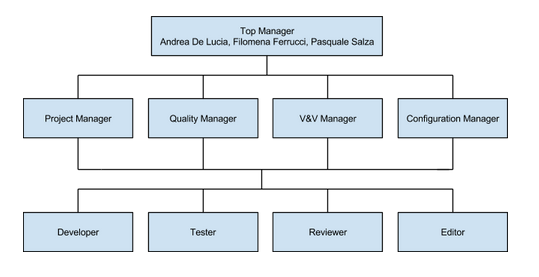
\includegraphics[scale=.7]{img/10.png}
\caption{Organizzazione team}
\label{fig:cd}
\end{figure*}
Si \`{e} deciso di stabilire il ruolo di un Verification \& Validation Manager in modo da garantire la redazione di checklist ad hoc per artefatto sulla base di quanto specificato nel QP.
Oltre alla definizione dei ruoli, nel QP \`{e} stato anche definito un Communication Plan. Questo definisce le modalit\`{a} di comunicazione tra i membri di tipo formale, ovvero tramite Google Groups.
Nel QP viene inoltre definito il workflow che la redazione dei documenti segue nel progetto. Il seguente grafico mostra lo schema adottato:
\begin{figure}[tp]
\centering
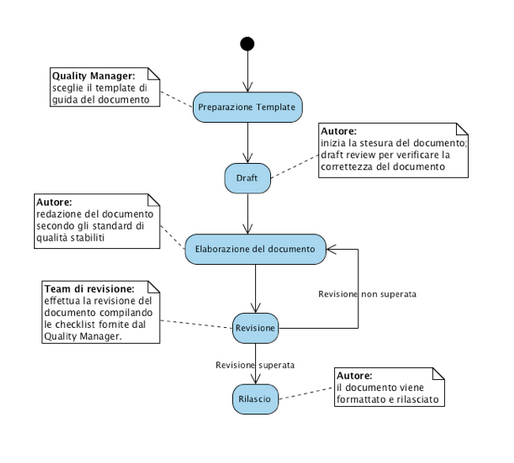
\includegraphics[scale=.5]{img/11.png}
\caption{Workflow qualit\`{a}}
\label{fig:cd}
\end{figure}
Compito del Quality Manager \`{e} quindi quello di definire dei Template da utilizzare per i documenti. Tali template sono quindi utilizzati dai membri del team nella redazione dei documenti.
In questo caso il documento viene definito come draft. Terminata l\rq elaborazione \`{e} compito del team di revisione predisposto effettuare una revisione formale del documento sulla base delle checklist preparate dal Quality Manager o dal V\& V Manager. 
Se tale revisione ha esito positivo il documento pu\`{o} essere rilasciato, altrimenti deve essere modificato rispettando quella che \`{e} la checklist compilata dal team di revisione predisposto.
Nel nostro caso il ruolo di team di revisione spetta ad uno o due membri designati dal project manager incaricati di rivedere un documento. Ovviamente nel team non rientra il membro redattore del documento in questione.
Si \`{e} deciso di specificare, in ogni documento, una revision history indicando redattore, data e tipologie di modifiche effettuate, una pagina di intestazione indicante titolo del documento, nome progetto, versione. 
Inoltre vengono indicati font da utilizzare, grandezza, tipologie di intestazioni di paragrafi etc.
Per quanto concerne il software al momento non sono state specificate modalit\`{a} di verifica dello stesso. Questo \`{e} dovuto alla non conoscenza delle tecnologie che saranno adoperate, in particolare C\# e l’ambiente .NET, per cui al momento non risulta facile prendere delle decisioni in merito.
Tuttavia, considerato che C\# presenta notevoli similitudini con il linguaggio Java si pu\`{o} pensare di utilizzare delle metriche statiche del codice oltre che delle metriche specifiche per linguaggi ad oggetti.
Sicuramente come parametro verr\`{a} tenuto in considerazione la presenza di commenti a metodi, classi e variabili ove queste non siano di immediata comprensione.
Per il reporting e l\rq issue tracking del codice si utilizzeranno i sistemi integrati in BitBucket che \`{e} la repository git utilizzata per il codice sorgente nell\rq ambito del progetto.
Dal momento che tale documento \`{e} stato redatto insieme col Risk Management Plan (RiMP) \`{e} risultato altrettanto rilevante includere in una apposita sezione del QP i rischi riguardanti la qualit\`{a} di progetto:
\begin{figure}[h]
\centering
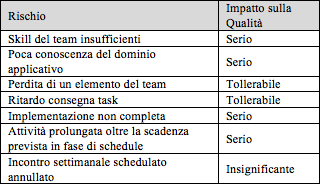
\includegraphics[scale=.7]{img/12.png}
\caption{Rischi}
\label{fig:cd}
\end{figure}
L\rq impatto sulla qualit\`{a} \`{e} riportato in categorie qualitative da Serio a Insignificante, dal pi\`{u} grave al meno grave.
Come gi\`{a} detto in precedenza, visto il legame tra Quality e Verification and Validation, i due plan sono stati redatti parallelamente.
Il V\& V Plan ha lo scopo di predisporre delle linee guida per la verifica e la validazione di un artefatto prima di essere definito baselined.
La fase di verifica e validazione degli artefatti prodotti durante lo sviluppo del sistema, prevede l\rq utilizzo di checklist di revisione. Per ogni artefatto sottoposto a revisione verr\`{a} definita una checklist specifica. 
Per cui vi sar\`{a} una fase di pianificazione in cui verranno elaborate le checklist e selezionati dei membri per la revisione, seguita da una fase di definition in cui vi sar\`{a} la realizzazione fisica del template della checklist, messo a disposizione di tutti.
Nella fase di review i revisori hanno il compito di verificare che l\rq artefatto sia conforme a quanto definito nel QP.
Se l\rq artefatto non \`{e} accettato allora vi \`{e} una fase di rework in cui esso deve essere adeguato rispetto a quanto stabilito nella checklist.
Il diagramma seguente riporta le fasi del processo di revisione degli artefatti prodotti nell\rq ambito del progetto del sistema:
\begin{figure}[h]
\centering
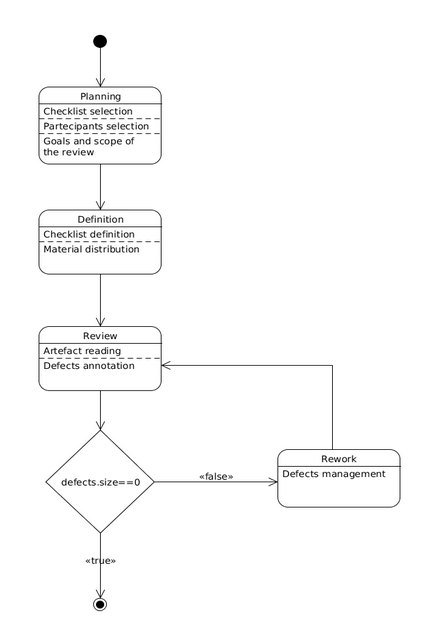
\includegraphics[scale=.6]{img/13.png}
\caption{Diagramma fasi di revisione}
\label{fig:cd}
\end{figure}
Alcune checklist vengono proposte in seguito nel documento. Ovviamente tali checklist e quindi monitoraggio degli artefatti, rientra nella normale esecuzione delle fasi del progetto cos\`{i} come descritto nel PMBOK 5 e nello specifico nella fase di Monitoring and Controlling.
Il QP e il VVP fanno s\`{i} che venga aggiornata la sezione 8 del SPMP nella quale rientrano informazioni sulla verifica e validazione e qualit\`{a}.
La rilevanza data all\rq aspetto della qualit\`{a} rientra nell\rq ottica dell\rq ottenimento di un prodotto che sia conforme a quelle che possano essere le aspettative dell\rq utente finale.
Inoltre consentir\`{a} una coerenza e consistenza per quanto riguarda lo scope di progetto, per cui deviazioni saranno evitate.
Aspetto negativo pu\`{o} essere l\rq introduzione di una eccessiva burocrazia in quello che dovrebbe essere uno sviluppo basato su tecniche agili. Tuttavia si far\`{a} in modo che tali processi di verifica non blocchino eccessivamente il processo di sviluppo del sistema.
Un ulteriore sforzo da parte del team \`{e} stato fatto per la creazione del Risk Management Plan (RiMP).
Seppur il progetto \`{e} di piccole dimensioni si \`{e} ritenuto fondamentale predisporre un piano per l\rq identificazione, la valutazione, il monitoraggio dei rischi.
Infatti nonostante la nostra breve esperienza dai precedenti corsi \`{e} subito risultato evidente come il sottovalutare dei rischi ha portato in seguito a problemi, come ritardi nei tempi di consegna o addirittura fine prematura del progetto.
Innanzitutto si \`{e} proceduto con l’individuare delle categorie di valutazione per quanto riguarda la probabilit\`{a} e l’impatto di un rischio.
Un primo meeting ci ha quindi portato a categorizzare la probabilit\`{a} di accadimento di un rischio e il suo impatto.
Attraverso una fase di brainstorming e benchmarking con progetti precedenti si sono identificati una serie di rischi da valutare. 
In un ulteriore meeting, un moderatore ha sottoposto ad ogni membro del team la lista dei rischi chiedendo di valutarne l’impatto e la probabilit\`{a}. Le risposte anonime, sono state raccolte effettuandone una convergenza verso valori unici.
Per alcuni rischi \`{e} stato necessaria altra discussione, per altri invece la convergenza era ampia. Questa tecnica viene definita come tecnica Delphi.
La risultante \`{e} la seguente tabella dei rischi:
\begin{figure}[h]
\centering
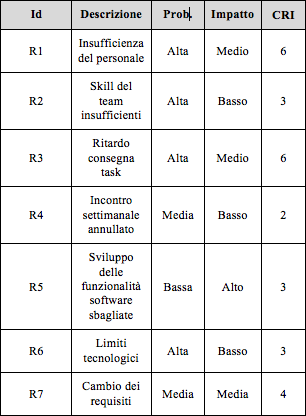
\includegraphics[scale=.6]{img/17.png}
\caption{Tabella dei rischi}
\label{fig:cd}
\end{figure}
Il rischio riguardante gli skills insufficienti \`{e} stato ritenuto di impatto basso in quanto i membri del team hanno effettuato un\rq autovalutazione asserendo di essere in grado di colmare il gap in tempi brevi. Questo supportato soprattutto dalla presenza di un corso di Sviluppo Applicazioni Mobili al secondo semestre.
Per ogni rischio \`{e} stato predisposto un breve piano di contingenza da attuare nel caso si verifichi e delle azioni per mitigare i trigger che scatenano i rischi. Vista la dimensione del progetto e l\rq assenza di un budget economico non si \`{e} ritenuto necessario predisporre piani dettagliati.
\begin{figure}[h]
\centering
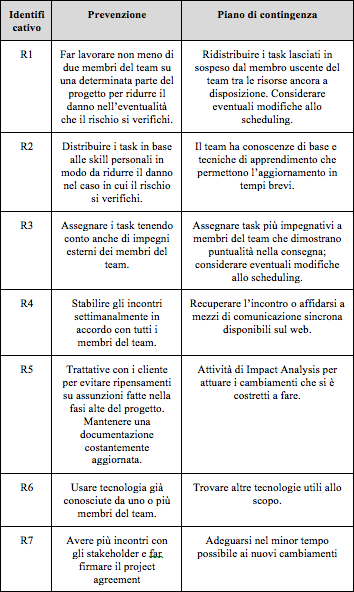
\includegraphics[scale=.6]{img/18.png}
\caption{Piano di contigenza}
\label{fig:cd}
\end{figure}
Il RiMP oltre a comportare un aggiornamento dell’SPMP ha permesso la creazione di un Risk Register (RiR) sul quale sono riportati i rischi da monitorare durante la fase di esecuzione del progetto.
Tale RiR verr\`{a} aggiornato costantemente mano a mano che il progetto progredisce, aggiornando sia la probabilit\`{a} di accadimento sia l\rq impatto.
Da quanto descritto finora si pu\`{o} notare come l’SPMP subisca modifiche mano a mano che i vari piani vengono elaborati. Altra sezione da considerare \`{e} la definizione della consegna del prodotto. Cos\`{i} come specificato sin dalla prima definizione dell’SPMP, il prodotto \`{e} dapprima prototipato con una versione web-based in cui sono presenti alcune funzionalit\`{a} di base, successivamente tale prototipo verr\`{a} evoluto creando la versione finale del sito web, accompagnata da un app principale per Windows Phone. Entrambe si interfacceranno con un web service restful.

\subsection{Esecuzione}
Durante la fase di esecuzione, cos\`{i} come definito nello scheduling, vengono elaborate le deliverables principali:\\
\begin{itemize}
\item SDD
\item ODD
\item Codice Sorgente:
\begin{itemize}
\item Web Service
\item App per Windows Phone
\item Web application
\end{itemize}
\item Database
\item Test Plan
\end{itemize}
La base di partenza \`{e} ovviamente tutta la documentazione di Management prodotta nella fase di Initiating e Planning. Fondamentale risulta il RAD da cui partire per una prima decomposizione del sistema in sottosistemi.
Questa fase verr\`{a} quindi descritta in dettaglio nella sezione riguardante il software in cui sono descritti i vari documenti riportati sopra tra cui il RAD.


\subsection{Monitoraggio e Controllo}
Il monitoraggio e controllo \`{e} una fase che ha inizio insieme alla fase di pianificazione e dura fino alla fase di chiusura, \`{e} una fase dove si valuta l’avanzamento dei lavori e si attua il piano che \`{e} stato concepito nel Verification \& Validation Plan seguendo le metriche di misurazione di qualit\`{a} definite nel Quality Plan. In pratica durante le fasi di pianificazione e esecuzione tramite l\rq utilizzo di checklist definite nel V \& V si revisionano i documenti creati. Vi sono diverse tipologie di checklist quelle per i documenti, dove vi \`{e} un componente del team che compila le checklist e quando termina invia le checklist al creatore del documento che la controlla e decide di accettarla e apportare le modifiche richieste. Di seguito il template utilizzato per la checklist di revisione dei documenti:\\

\begin{figure}[h]
\centering
\includegraphics[scale=.5]{img/checklist.png}
\caption{Checklist valutazione generica documento}
\end{figure}

Altre tipologie di checklist che abbiamo definito sono per la raccolta e analisi dei requisiti, stima dei costi e dei tempi, software configuration management, risk management, quality assurance e  testing. La compilazione di queste checklist da parte del team porta a una chiara misurazione della qualit\`{a} del progetto, per maggiori dettagli sulle checklist invito a consultare il documento Verification \& Validation Plan. Dopo questa analisi che ci ha permesso di monitorare il progetto sono stati redatti dei management e quality report per capire appunto cosa doveva essere revisionato e aggiornato, un esempio nel quality report:\\
 
\begin{figure}[!h]
\centering
\includegraphics[scale=.5]{img/risultato.png}
\caption{Risultato Checklist specifica}
\end{figure}

Dove B sta a indicare che il documento \`{e} stato accettato ma vanno apportate lievi modifiche.

\subsection{Chiusura}
Una volta che arriveremo alla fase di chiusura di progetto e quindi aver ottenuto il risultato sulla base delle specifiche date in input, si proceder\`{a} con la stesura della post-mortem review ovvero un deliverable per analizzare gli elementi del progetto e capire se sono stati di successo o di insuccesso. Dopo aver dato il proprio giudizio vi sono una serie di domande aperte che riguardano lesson learned e considerazioni finali.
La post-mortem review ci aiuter\`{a} nel gestire futuri rischi gi\`{a} incotrati in questo progetto quindi migliorando le nostre skill dal punto di vista del risk management e delle Best Practice.
